\documentclass[11pt]{report}

\usepackage[utf8]{inputenc}

%%% PAGE DIMENSIONS
\usepackage{geometry} % to change the page dimensions
\geometry{a4paper} % or letterpaper (US) or a5paper or....
\geometry{top=2.5cm}
\geometry{right=2.5cm}
\geometry{bottom=2cm}
\geometry{left=2.5cm}

\usepackage{graphicx}
\usepackage{amsmath}
\usepackage{amssymb}
\usepackage{csquotes}
\usepackage{hyperref}
\usepackage[nonumberlist]{glossaries}  
\usepackage{titlesec}
\usepackage[normalem]{ulem}
\usepackage{nameref}
\usepackage{pdfpages}
\usepackage{framed}
\usepackage[ngerman]{babel}
\usepackage[T1]{fontenc}
\usepackage{booktabs}
\usepackage{array}
\usepackage{paralist}
\usepackage{verbatim}
\usepackage{subfig}
\usepackage{multicol}
\usepackage{caption}
\usepackage{footnote}
\usepackage{listings}
\usepackage{color}
\usepackage{selinput}
\usepackage{float}
\SelectInputMappings{
	adieresis={ä},
	germandbls={ß}
}
\usepackage{babel}
\usepackage{ulem}


% Spezialpakete

\usepackage{tikz}
% TikZ-Bibliotheken
\usetikzlibrary{arrows}
\usetikzlibrary{shapes}
\usetikzlibrary{decorations.pathmorphing}
\usetikzlibrary{decorations.pathreplacing}
\usetikzlibrary{decorations.shapes}
\usetikzlibrary{decorations.text}


%%% HEADERS & FOOTERS
\usepackage{fancyhdr}
\pagestyle{fancy}
\renewcommand{\headrulewidth}{0pt}
\lhead{}\chead{}\rhead{}
\lfoot{}\cfoot{\thepage}\rfoot{}
\usepackage[default,osfigures,scale=0.95]{opensans} %% 
\usepackage[T1]{fontenc}

%%% ToC (table of contents) APPEARANCE
\usepackage[nottoc,notlof,notlot]{tocbibind}
\usepackage[titles,subfigure]{tocloft}
\renewcommand{\cftsecfont}{\rmfamily\mdseries\upshape}
\renewcommand{\cftsecpagefont}{\rmfamily\mdseries\upshape}

\newcommand{\HRule}[1]{\rule{\linewidth}{#1}} 	% Horizontal rule

%%%%%%%%%%%%%%%%%%%%%%%%%%%%%%
\titleformat{\chapter}{\normalfont\huge}{\thechapter.}{20pt}{\huge\it}

\begin{document}
	\begin{titlepage}
		\begin{center}
			\textsc{\Large Spezifikation}\\
			
			% Title
			{ \huge \bfseries Flexible ALU \\[0.4cm] }
			\HRule{0.5pt} \\[2.5cm]			
		\end{center}
		
		\begin{table}[h]
			\centering
			\begin{tabular}{l|l|l}
				\multicolumn{1}{c|}{\Large \textbf{  Version  }} & \multicolumn{1}{c|}{\Large \textbf{  Bearbeiter  }} & \multicolumn{1}{c}{\Large \textbf{  Neuerung  }} \\ \hline
				\multicolumn{1}{c|}{1.0}              & \multicolumn{1}{c|}{}                    & \multicolumn{1}{c}{}                  \\
				&                                          &                                       \\
				&                                          &                                      
			\end{tabular}
		\end{table}
		
		\vfill
		\begin{flushright}
			HFI414\\
			Q1 2016\\
			Torben Voltmer\\
			Sarah Wöckener\\
		\end{flushright}
	\end{titlepage}
	%%%%%%%%%%%%%%%%%%%%%%%%%%%%%%%%%%%
	\tableofcontents
	
	\pagebreak
	%%%%%%%%%%%%%%%%%%%%%%%%%%%%%%%%%%%
	
	\chapter{Datenblatt}
	
	\section{Einsatzbereich}
	
	\section{Features}
	
	\section{Funktion}
	\begin{table}[h]
		\centering
		\label{codierungstabelle}
		\begin{tabular}{|lll|l|}
			\hline
			\multicolumn{3}{|c|}{CMD}                            & \multicolumn{1}{c|}{}             \\
			\multicolumn{1}{|l|}{2} & \multicolumn{1}{l|}{1} & 0 & Logisch/arithmetischer Ausdruck \\ \hline
			0                       & 0                      & 0 & AND                               \\ \hline
			0                       & 0                      & 1 & OR                                \\ \hline
			0                       & 1                      & 0 & NOT                               \\ \hline
			0                       & 1                      & 1 & ADD                               \\ \hline
			1                       & 0                      & 0 & SUB                               \\ \hline
			1                       & 0                      & 1 & MUL                               \\ \hline
			1                       & 1                      & 0 & MC0                               \\ \hline
			1                       & 1                      & 1 & MC1                               \\ \hline
		\end{tabular}
		\caption{Befehls-Codierung}
	\end{table}
	
	
	
	\section{Blockschaltbild}
	\begin{figure}[htbp]
		\begin{center}
			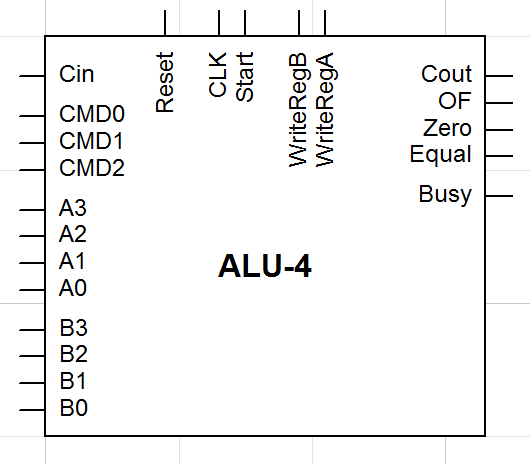
\includegraphics[]{aeusseresBlockschaltbild}
			\label{aeusseresBlockschaltbild}
			\caption{Äußeres Blockschaltbild}
		\end{center}
	\end{figure}
	
	
	
	\section{Schnittstellen}
	Siehe Seite \pageref{portliste}.
	\begin{table}[]
		\centering
		\label{portliste}
		\begin{tabular}{|l|l|l|}
			\hline
			Port & Typ & Funktion \\ \hline\hline
			
			Cin & Input &  \\ \hline
			
			WriteRegA & Input & Wenn 1, wird Operand 1 in Register A geschrieben (solange die Arbitierung außen liegt). \\ \hline
			
			WriteRegB & Input & Wenn 1, wird Operand 2 in Register B geschrieben. \\ \hline
			
			Reset & Input & Register werden zurückgesetzt. \\ \hline
			
			Start & Input & Die Operation wird mit den angelegten Operanden durchgeführt. \\ \hline
			
			CLK & Input & Takt. \\ \hline
			
			CMD0..2 & Input & Auswahl des Befehls. Codierung siehe S. \pageref{codierungstabelle} \\ \hline
			
			A0..3 & Bidirektional & \begin{tabular}[c]{@{}l@{}}IN: Operand 1 wird mit WriteRegA angelegt.\\ OUT: Ist Busy 0, liegt hier das Ergebnis der Berechnung an.\\ Die Subtraktion liefert das 2er-Komplement.\\ Multiplikation liefert hier die LSBits des Ergebnisses.\end{tabular} \\ \hline
			
			B0..3 & Bidirektional & \begin{tabular}[c]{@{}l@{}}IN: Operand 2 wird mit WriteRegB angelegt.\\ OUT: Wird Busy 0, liegt hier 0 an,\\ die Multiplikation liefert hier die MSBits des Ergebnisses.\end{tabular} \\ \hline
			
			Busy & Output & \begin{tabular}[c]{@{}l@{}}Ist 1, solange die ALU arbeitet.\\ Wird Busy 0, liegt das Ergebnis an A0..3 und B0..3 an.\end{tabular} \\ \hline
			
			OF & Output & \begin{tabular}[c]{@{}l@{}}OF ist 1, wenn die letzten beiden Übertragsbits ungleich sind\\ und somit ein Overflow auftritt.\end{tabular} \\ \hline
			
			Zero & Output & Zero ist 1, wenn alle Ergebnisbits 0 sind. \\ \hline
			
			Equal & Output & Equal ist 1, wenn die 4 Ergebnisbits von A und B bitweise gleich sind. \\ \hline
			
			Cout & Output & \begin{tabular}[c]{@{}l@{}}Tritt während der Berechnung ein Übertrag über die letzte Bitstelle auf,\\ wird Cout 1 und kann weiter behandelt werden.\end{tabular} \\ \hline
		\end{tabular}
		\caption{Liste aller Ports}
	\end{table}
	
	\colorbox{red}{flags}
	hahaa
	
	\section{Gate-Count}
	Für eine detaillierte Angabe der Gatteräquivalente siehe S. \pageref{gatecounttable}.
	\begin{table}[]
		\centering
		\label{gatecounttable}
		\begin{tabular}{llll}
			\hline
			Typ                                          & Gatteräquivalente          & Anzahl                  & Summe                      \\ \hline\hline
			\multicolumn{1}{|l}{Gatter}                  &                            &                         & \multicolumn{1}{l|}{}      \\ \hline
			\multicolumn{1}{|l|}{AND2}                   & \multicolumn{1}{l|}{1,5}   & \multicolumn{1}{l|}{65} & \multicolumn{1}{l|}{97,5}  \\ \hline
			\multicolumn{1}{|l|}{AND3}                   & \multicolumn{1}{l|}{2}     & \multicolumn{1}{l|}{13} & \multicolumn{1}{l|}{26}    \\ \hline
			\multicolumn{1}{|l|}{AND4}                   & \multicolumn{1}{l|}{2,5}   & \multicolumn{1}{l|}{12} & \multicolumn{1}{l|}{30}    \\ \hline
			\multicolumn{1}{|l|}{AND5}                   & \multicolumn{1}{l|}{3}     & \multicolumn{1}{l|}{4}  & \multicolumn{1}{l|}{12}    \\ \hline
			\multicolumn{1}{|l|}{Inv}                    & \multicolumn{1}{l|}{0,5}   & \multicolumn{1}{l|}{11} & \multicolumn{1}{l|}{5,5}   \\ \hline
			\multicolumn{1}{|l|}{Mult2:1}                & \multicolumn{1}{l|}{3}     & \multicolumn{1}{l|}{28} & \multicolumn{1}{l|}{84}    \\ \hline
			\multicolumn{1}{|l|}{Mult4:1}                & \multicolumn{1}{l|}{7}     & \multicolumn{1}{l|}{0}  & \multicolumn{1}{l|}{0}     \\ \hline
			\multicolumn{1}{|l|}{Mult8:1}                & \multicolumn{1}{l|}{16}    & \multicolumn{1}{l|}{9}  & \multicolumn{1}{l|}{144}   \\ \hline
			\multicolumn{1}{|l|}{NAND2}                  & \multicolumn{1}{l|}{1}     & \multicolumn{1}{l|}{6}  & \multicolumn{1}{l|}{6}     \\ \hline
			\multicolumn{1}{|l|}{NAND3}                  & \multicolumn{1}{l|}{1,5}   & \multicolumn{1}{l|}{0}  & \multicolumn{1}{l|}{0}     \\ \hline
			\multicolumn{1}{|l|}{NAND4}                  & \multicolumn{1}{l|}{2}     & \multicolumn{1}{l|}{0}  & \multicolumn{1}{l|}{0}     \\ \hline
			\multicolumn{1}{|l|}{NAND6}                  & \multicolumn{1}{l|}{4,5}   & \multicolumn{1}{l|}{0}  & \multicolumn{1}{l|}{0}     \\ \hline
			\multicolumn{1}{|l|}{NAND8}                  & \multicolumn{1}{l|}{5,5}   & \multicolumn{1}{l|}{0}  & \multicolumn{1}{l|}{0}     \\ \hline
			\multicolumn{1}{|l|}{NOR2}                   & \multicolumn{1}{l|}{1}     & \multicolumn{1}{l|}{0}  & \multicolumn{1}{l|}{0}     \\ \hline
			\multicolumn{1}{|l|}{NOR3}                   & \multicolumn{1}{l|}{1,5}   & \multicolumn{1}{l|}{0}  & \multicolumn{1}{l|}{0}     \\ \hline
			\multicolumn{1}{|l|}{NOR4}                   & \multicolumn{1}{l|}{2}     & \multicolumn{1}{l|}{0}  & \multicolumn{1}{l|}{0}     \\ \hline
			\multicolumn{1}{|l|}{OR2}                    & \multicolumn{1}{l|}{1,5}   & \multicolumn{1}{l|}{21} & \multicolumn{1}{l|}{31,5}  \\ \hline
			\multicolumn{1}{|l|}{OR3}                    & \multicolumn{1}{l|}{2}     & \multicolumn{1}{l|}{4}  & \multicolumn{1}{l|}{8}     \\ \hline
			\multicolumn{1}{|l|}{OR4}                    & \multicolumn{1}{l|}{2,5}   & \multicolumn{1}{l|}{9}  & \multicolumn{1}{l|}{22,5}  \\ \hline
			\multicolumn{1}{|l|}{OR5}                    & \multicolumn{1}{l|}{3}     & \multicolumn{1}{l|}{4}  & \multicolumn{1}{l|}{12}    \\ \hline
			\multicolumn{1}{|l|}{XNOR2}                  & \multicolumn{1}{l|}{3}     & \multicolumn{1}{l|}{0}  & \multicolumn{1}{l|}{0}     \\ \hline
			\multicolumn{1}{|l|}{XOR2}                   & \multicolumn{1}{l|}{3}     & \multicolumn{1}{l|}{32} & \multicolumn{1}{l|}{96}    \\ \hline
			\multicolumn{1}{|l}{Speicher (Angabe / bit)} &                            &                         & \multicolumn{1}{l|}{}      \\ \hline
			\multicolumn{1}{|l|}{DFF}                    & \multicolumn{1}{l|}{7}     & \multicolumn{1}{l|}{4}  & \multicolumn{1}{l|}{28}    \\ \hline
			\multicolumn{1}{|l|}{DFF-R}                  & \multicolumn{1}{l|}{8}     & \multicolumn{1}{l|}{0}  & \multicolumn{1}{l|}{0}     \\ \hline
			\multicolumn{1}{|l|}{DFF-S}                  & \multicolumn{1}{l|}{8}     & \multicolumn{1}{l|}{0}  & \multicolumn{1}{l|}{0}     \\ \hline
			\multicolumn{1}{|l|}{DFF-SR}                 & \multicolumn{1}{l|}{9}     & \multicolumn{1}{l|}{0}  & \multicolumn{1}{l|}{0}     \\ \hline
			\multicolumn{1}{|l|}{DRAM}                   & \multicolumn{1}{l|}{5}     & \multicolumn{1}{l|}{0}  & \multicolumn{1}{l|}{0}     \\ \hline
			\multicolumn{1}{|l|}{DRAM (o. Anst.)}        & \multicolumn{1}{l|}{0,25}  & \multicolumn{1}{l|}{0}  & \multicolumn{1}{l|}{0}     \\ \hline
			\multicolumn{1}{|l|}{SRAM}                   & \multicolumn{1}{l|}{7,5}   & \multicolumn{1}{l|}{0}  & \multicolumn{1}{l|}{0}     \\ \hline
			\multicolumn{1}{|l|}{SRAM (o. Anst.)}        & \multicolumn{1}{l|}{1}     & \multicolumn{1}{l|}{0}  & \multicolumn{1}{l|}{0}     \\ \hline
			\multicolumn{1}{|l|}{Buffer4}                & \multicolumn{1}{l|}{4}     & \multicolumn{1}{l|}{19} & \multicolumn{1}{l|}{76}    \\ \hline
			\multicolumn{1}{|l|}{74\_181}                & \multicolumn{1}{l|}{108,5} & \multicolumn{1}{l|}{1}  & \multicolumn{1}{l|}{108,5} \\ \hline\hline
			Gesamtsumme:                                 &                            &                         & 787,5                      \\ \hline
		\end{tabular}
		\caption{Gatteräquivalente}
	\end{table}
	
	
	\section{Timing-Diagramm}
	\section{Leistungsabschätzung}
	watt pro gatter pro mhz als energieverbrauch
	
	
	\chapter{Spezifikation}
	
	\section{Register}
	\subsection{RegA}
	Register für Operand A und das low-nibble des Ergebnisses.
	Es handelt sich um ein Bi-Reg-4.
	Die Arbitrierung des Registers liegt intern, solange busy=0 ist.
	Das Ergebnis liegt am Ausgang an, sobald busy=0 wird.
	
	\subsection{RegB}
	Analog zu RegA
	
	\subsection{AccuA}
	Akkumulatorregister für das low-nibble des Ergebnisses.
	Es handelt sich um ein Uni-Reg 4.
	Die Ausgänge des Registers können als Operand A verwendet werden.
	
	\subsection{AccuB}
	Analog zu AccuB
	
	\subsection{CMD}
	Register für den Befehlscode.
	Es handelt sich um ein Uni-Reg-3. Wir geschrieben sobald Start=1 gesetzt wird.
	
	\subsection{Flags}
	Register für die Flags.
	Es handelt sich um ein Uni-Reg-4.
	Die Flags liegen am Ausgang an, sobald busy=0 wird.
	
	
	\section{Modul-Beschreibung}
	\subsection{74\_181}
	\subsection{MUL-4}
	\subsection{Barrel-Shifter-8}
	\subsection{Bi-Reg-n}
	\subsection{Uni-Reg-n}
	\subsection{MC-PROM}
	\subsubsection{Programmierung}
	
	\section{Detailblockschaltbild}
	Für das innere Schaltbild siehe Seite \pageref{inneresBlockschaltbild}.
	\begin{figure}[htbp]
		\begin{center}
			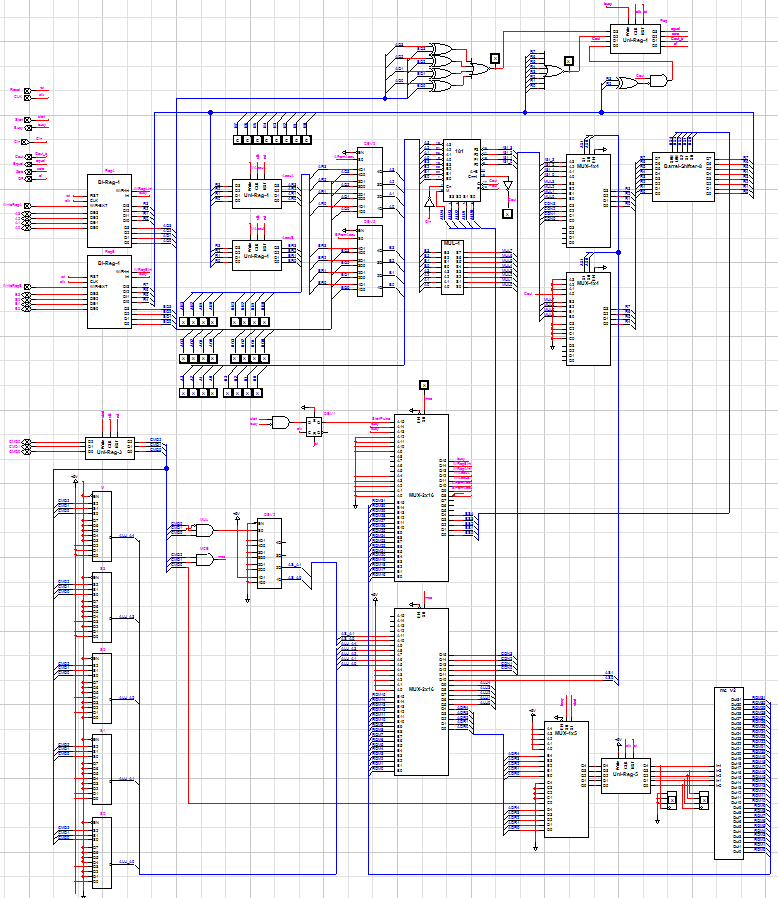
\includegraphics[width=\textwidth]{inneresBlockschaltbild}
			\label{inneresBlockschaltbild}
			\caption{Inneres Blockschaltbild}
		\end{center}
	\end{figure}
	
\end{document}\documentclass[11pt]{report}

\usepackage[utf8]{inputenc}

%%% PAGE DIMENSIONS
\usepackage{geometry} % to change the page dimensions
\geometry{a4paper} % or letterpaper (US) or a5paper or....
\geometry{top=2.5cm}
\geometry{right=2.5cm}
\geometry{bottom=2cm}
\geometry{left=2.5cm}

\usepackage{graphicx}
\usepackage{amsmath}
\usepackage{amssymb}
\usepackage{csquotes}
\usepackage{hyperref}
\usepackage[nonumberlist]{glossaries}  
\usepackage{titlesec}
\usepackage[normalem]{ulem}
\usepackage{nameref}
\usepackage{pdfpages}
\usepackage{framed}
\usepackage[ngerman]{babel}
\usepackage[T1]{fontenc}
\usepackage{booktabs}
\usepackage{array}
\usepackage{paralist}
\usepackage{verbatim}
\usepackage{subfig}
\usepackage{multicol}
\usepackage{caption}
\usepackage{footnote}
\usepackage{listings}
\usepackage{color}
\usepackage{selinput}
\usepackage{float}
\SelectInputMappings{
	adieresis={ä},
	germandbls={ß}
}
\usepackage{babel}
\usepackage{ulem}


% Spezialpakete

\usepackage{tikz}
% TikZ-Bibliotheken
\usetikzlibrary{arrows}
\usetikzlibrary{shapes}
\usetikzlibrary{decorations.pathmorphing}
\usetikzlibrary{decorations.pathreplacing}
\usetikzlibrary{decorations.shapes}
\usetikzlibrary{decorations.text}


%%% HEADERS & FOOTERS
\usepackage{fancyhdr}
\pagestyle{fancy}
\renewcommand{\headrulewidth}{0pt}
\lhead{}\chead{}\rhead{}
\lfoot{}\cfoot{\thepage}\rfoot{}
\usepackage[default,osfigures,scale=0.95]{opensans} %% 
\usepackage[T1]{fontenc}

%%% ToC (table of contents) APPEARANCE
\usepackage[nottoc,notlof,notlot]{tocbibind}
\usepackage[titles,subfigure]{tocloft}
\renewcommand{\cftsecfont}{\rmfamily\mdseries\upshape}
\renewcommand{\cftsecpagefont}{\rmfamily\mdseries\upshape}

\newcommand{\HRule}[1]{\rule{\linewidth}{#1}} 	% Horizontal rule

%%%%%%%%%%%%%%%%%%%%%%%%%%%%%%
\titleformat{\chapter}{\normalfont\huge}{\thechapter.}{20pt}{\huge\it}

\begin{document}
	\begin{titlepage}
		\begin{center}
			\textsc{\Large Spezifikation}\\
			
			% Title
			{ \huge \bfseries Flexible ALU \\[0.4cm] }
			\HRule{0.5pt} \\[2.5cm]			
		\end{center}
		
		\begin{table}[h]
			\centering
			\begin{tabular}{l|l|l}
				\multicolumn{1}{c|}{\Large \textbf{  Version  }} & \multicolumn{1}{c|}{\Large \textbf{  Bearbeiter  }} & \multicolumn{1}{c}{\Large \textbf{  Neuerung  }} \\ \hline
				\multicolumn{1}{c|}{1.0}              & \multicolumn{1}{c|}{}                    & \multicolumn{1}{c}{}                  \\
				&                                          &                                       \\
				&                                          &                                      
			\end{tabular}
		\end{table}
		
		\vfill
		\begin{flushright}
			HFI414\\
			Q1 2016\\
			Torben Voltmer\\
			Sarah Wöckener\\
		\end{flushright}
	\end{titlepage}
	%%%%%%%%%%%%%%%%%%%%%%%%%%%%%%%%%%%
	\tableofcontents
	
	\pagebreak
	%%%%%%%%%%%%%%%%%%%%%%%%%%%%%%%%%%%
	
	\chapter{Datenblatt}
	
	\section{Einsatzbereich}
	
	\section{Features}
	
	\section{Funktion}
	\begin{table}[h]
		\centering
		\label{codierungstabelle}
		\begin{tabular}{|lll|l|}
			\hline
			\multicolumn{3}{|c|}{CMD}                            & \multicolumn{1}{c|}{}             \\
			\multicolumn{1}{|l|}{2} & \multicolumn{1}{l|}{1} & 0 & Logisch/arithmetischer Ausdruck \\ \hline
			0                       & 0                      & 0 & AND                               \\ \hline
			0                       & 0                      & 1 & OR                                \\ \hline
			0                       & 1                      & 0 & NOT                               \\ \hline
			0                       & 1                      & 1 & ADD                               \\ \hline
			1                       & 0                      & 0 & SUB                               \\ \hline
			1                       & 0                      & 1 & MUL                               \\ \hline
			1                       & 1                      & 0 & MC0                               \\ \hline
			1                       & 1                      & 1 & MC1                               \\ \hline
		\end{tabular}
		\caption{Befehls-Codierung}
	\end{table}
	
	
	
	\section{Blockschaltbild}
	\begin{figure}[htbp]
		\begin{center}
			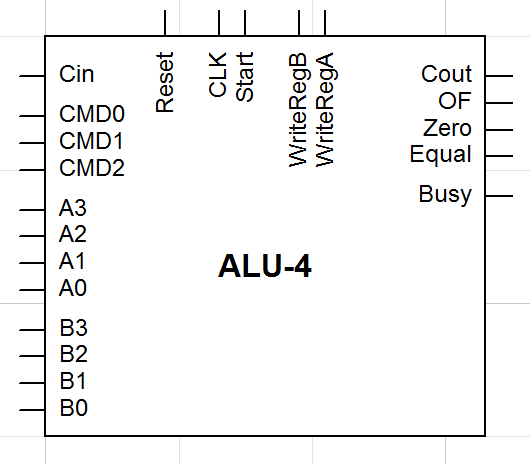
\includegraphics[]{aeusseresBlockschaltbild}
			\label{aeusseresBlockschaltbild}
			\caption{Äußeres Blockschaltbild}
		\end{center}
	\end{figure}
	
	
	
	\section{Schnittstellen}
	Siehe Seite \pageref{portliste}.
	\begin{table}[]
		\centering
		\label{portliste}
		\begin{tabular}{|l|l|l|}
			\hline
			Port & Typ & Funktion \\ \hline\hline
			
			Cin & Input &  \\ \hline
			
			WriteRegA & Input & Wenn 1, wird Operand 1 in Register A geschrieben (solange die Arbitierung außen liegt). \\ \hline
			
			WriteRegB & Input & Wenn 1, wird Operand 2 in Register B geschrieben. \\ \hline
			
			Reset & Input & Register werden zurückgesetzt. \\ \hline
			
			Start & Input & Die Operation wird mit den angelegten Operanden durchgeführt. \\ \hline
			
			CLK & Input & Takt. \\ \hline
			
			CMD0..2 & Input & Auswahl des Befehls. Codierung siehe S. \pageref{codierungstabelle} \\ \hline
			
			A0..3 & Bidirektional & \begin{tabular}[c]{@{}l@{}}IN: Operand 1 wird mit WriteRegA angelegt.\\ OUT: Ist Busy 0, liegt hier das Ergebnis der Berechnung an.\\ Die Subtraktion liefert das 2er-Komplement.\\ Multiplikation liefert hier die LSBits des Ergebnisses.\end{tabular} \\ \hline
			
			B0..3 & Bidirektional & \begin{tabular}[c]{@{}l@{}}IN: Operand 2 wird mit WriteRegB angelegt.\\ OUT: Wird Busy 0, liegt hier 0 an,\\ die Multiplikation liefert hier die MSBits des Ergebnisses.\end{tabular} \\ \hline
			
			Busy & Output & \begin{tabular}[c]{@{}l@{}}Ist 1, solange die ALU arbeitet.\\ Wird Busy 0, liegt das Ergebnis an A0..3 und B0..3 an.\end{tabular} \\ \hline
			
			OF & Output & \begin{tabular}[c]{@{}l@{}}OF ist 1, wenn die letzten beiden Übertragsbits ungleich sind\\ und somit ein Overflow auftritt.\end{tabular} \\ \hline
			
			Zero & Output & Zero ist 1, wenn alle Ergebnisbits 0 sind. \\ \hline
			
			Equal & Output & Equal ist 1, wenn die 4 Ergebnisbits von A und B bitweise gleich sind. \\ \hline
			
			Cout & Output & \begin{tabular}[c]{@{}l@{}}Tritt während der Berechnung ein Übertrag über die letzte Bitstelle auf,\\ wird Cout 1 und kann weiter behandelt werden.\end{tabular} \\ \hline
		\end{tabular}
		\caption{Liste aller Ports}
	\end{table}
	
	\colorbox{red}{flags}
	hahaa
	
	\section{Gate-Count}
	Für eine detaillierte Angabe der Gatteräquivalente siehe S. \pageref{gatecounttable}.
	\begin{table}[]
		\centering
		\label{gatecounttable}
		\begin{tabular}{llll}
			\hline
			Typ                                          & Gatteräquivalente          & Anzahl                  & Summe                      \\ \hline\hline
			\multicolumn{1}{|l}{Gatter}                  &                            &                         & \multicolumn{1}{l|}{}      \\ \hline
			\multicolumn{1}{|l|}{AND2}                   & \multicolumn{1}{l|}{1,5}   & \multicolumn{1}{l|}{65} & \multicolumn{1}{l|}{97,5}  \\ \hline
			\multicolumn{1}{|l|}{AND3}                   & \multicolumn{1}{l|}{2}     & \multicolumn{1}{l|}{13} & \multicolumn{1}{l|}{26}    \\ \hline
			\multicolumn{1}{|l|}{AND4}                   & \multicolumn{1}{l|}{2,5}   & \multicolumn{1}{l|}{12} & \multicolumn{1}{l|}{30}    \\ \hline
			\multicolumn{1}{|l|}{AND5}                   & \multicolumn{1}{l|}{3}     & \multicolumn{1}{l|}{4}  & \multicolumn{1}{l|}{12}    \\ \hline
			\multicolumn{1}{|l|}{Inv}                    & \multicolumn{1}{l|}{0,5}   & \multicolumn{1}{l|}{11} & \multicolumn{1}{l|}{5,5}   \\ \hline
			\multicolumn{1}{|l|}{Mult2:1}                & \multicolumn{1}{l|}{3}     & \multicolumn{1}{l|}{28} & \multicolumn{1}{l|}{84}    \\ \hline
			\multicolumn{1}{|l|}{Mult4:1}                & \multicolumn{1}{l|}{7}     & \multicolumn{1}{l|}{0}  & \multicolumn{1}{l|}{0}     \\ \hline
			\multicolumn{1}{|l|}{Mult8:1}                & \multicolumn{1}{l|}{16}    & \multicolumn{1}{l|}{9}  & \multicolumn{1}{l|}{144}   \\ \hline
			\multicolumn{1}{|l|}{NAND2}                  & \multicolumn{1}{l|}{1}     & \multicolumn{1}{l|}{6}  & \multicolumn{1}{l|}{6}     \\ \hline
			\multicolumn{1}{|l|}{NAND3}                  & \multicolumn{1}{l|}{1,5}   & \multicolumn{1}{l|}{0}  & \multicolumn{1}{l|}{0}     \\ \hline
			\multicolumn{1}{|l|}{NAND4}                  & \multicolumn{1}{l|}{2}     & \multicolumn{1}{l|}{0}  & \multicolumn{1}{l|}{0}     \\ \hline
			\multicolumn{1}{|l|}{NAND6}                  & \multicolumn{1}{l|}{4,5}   & \multicolumn{1}{l|}{0}  & \multicolumn{1}{l|}{0}     \\ \hline
			\multicolumn{1}{|l|}{NAND8}                  & \multicolumn{1}{l|}{5,5}   & \multicolumn{1}{l|}{0}  & \multicolumn{1}{l|}{0}     \\ \hline
			\multicolumn{1}{|l|}{NOR2}                   & \multicolumn{1}{l|}{1}     & \multicolumn{1}{l|}{0}  & \multicolumn{1}{l|}{0}     \\ \hline
			\multicolumn{1}{|l|}{NOR3}                   & \multicolumn{1}{l|}{1,5}   & \multicolumn{1}{l|}{0}  & \multicolumn{1}{l|}{0}     \\ \hline
			\multicolumn{1}{|l|}{NOR4}                   & \multicolumn{1}{l|}{2}     & \multicolumn{1}{l|}{0}  & \multicolumn{1}{l|}{0}     \\ \hline
			\multicolumn{1}{|l|}{OR2}                    & \multicolumn{1}{l|}{1,5}   & \multicolumn{1}{l|}{21} & \multicolumn{1}{l|}{31,5}  \\ \hline
			\multicolumn{1}{|l|}{OR3}                    & \multicolumn{1}{l|}{2}     & \multicolumn{1}{l|}{4}  & \multicolumn{1}{l|}{8}     \\ \hline
			\multicolumn{1}{|l|}{OR4}                    & \multicolumn{1}{l|}{2,5}   & \multicolumn{1}{l|}{9}  & \multicolumn{1}{l|}{22,5}  \\ \hline
			\multicolumn{1}{|l|}{OR5}                    & \multicolumn{1}{l|}{3}     & \multicolumn{1}{l|}{4}  & \multicolumn{1}{l|}{12}    \\ \hline
			\multicolumn{1}{|l|}{XNOR2}                  & \multicolumn{1}{l|}{3}     & \multicolumn{1}{l|}{0}  & \multicolumn{1}{l|}{0}     \\ \hline
			\multicolumn{1}{|l|}{XOR2}                   & \multicolumn{1}{l|}{3}     & \multicolumn{1}{l|}{32} & \multicolumn{1}{l|}{96}    \\ \hline
			\multicolumn{1}{|l}{Speicher (Angabe / bit)} &                            &                         & \multicolumn{1}{l|}{}      \\ \hline
			\multicolumn{1}{|l|}{DFF}                    & \multicolumn{1}{l|}{7}     & \multicolumn{1}{l|}{4}  & \multicolumn{1}{l|}{28}    \\ \hline
			\multicolumn{1}{|l|}{DFF-R}                  & \multicolumn{1}{l|}{8}     & \multicolumn{1}{l|}{0}  & \multicolumn{1}{l|}{0}     \\ \hline
			\multicolumn{1}{|l|}{DFF-S}                  & \multicolumn{1}{l|}{8}     & \multicolumn{1}{l|}{0}  & \multicolumn{1}{l|}{0}     \\ \hline
			\multicolumn{1}{|l|}{DFF-SR}                 & \multicolumn{1}{l|}{9}     & \multicolumn{1}{l|}{0}  & \multicolumn{1}{l|}{0}     \\ \hline
			\multicolumn{1}{|l|}{DRAM}                   & \multicolumn{1}{l|}{5}     & \multicolumn{1}{l|}{0}  & \multicolumn{1}{l|}{0}     \\ \hline
			\multicolumn{1}{|l|}{DRAM (o. Anst.)}        & \multicolumn{1}{l|}{0,25}  & \multicolumn{1}{l|}{0}  & \multicolumn{1}{l|}{0}     \\ \hline
			\multicolumn{1}{|l|}{SRAM}                   & \multicolumn{1}{l|}{7,5}   & \multicolumn{1}{l|}{0}  & \multicolumn{1}{l|}{0}     \\ \hline
			\multicolumn{1}{|l|}{SRAM (o. Anst.)}        & \multicolumn{1}{l|}{1}     & \multicolumn{1}{l|}{0}  & \multicolumn{1}{l|}{0}     \\ \hline
			\multicolumn{1}{|l|}{Buffer4}                & \multicolumn{1}{l|}{4}     & \multicolumn{1}{l|}{19} & \multicolumn{1}{l|}{76}    \\ \hline
			\multicolumn{1}{|l|}{74\_181}                & \multicolumn{1}{l|}{108,5} & \multicolumn{1}{l|}{1}  & \multicolumn{1}{l|}{108,5} \\ \hline\hline
			Gesamtsumme:                                 &                            &                         & 787,5                      \\ \hline
		\end{tabular}
		\caption{Gatteräquivalente}
	\end{table}
	
	
	\section{Timing-Diagramm}
	\section{Leistungsabschätzung}
	watt pro gatter pro mhz als energieverbrauch
	
	
	\chapter{Spezifikation}
	
	\section{Register}
	\subsection{RegA}
	Register für Operand A und das low-nibble des Ergebnisses.
	Es handelt sich um ein Bi-Reg-4.
	Die Arbitrierung des Registers liegt intern, solange busy=0 ist.
	Das Ergebnis liegt am Ausgang an, sobald busy=0 wird.
	
	\subsection{RegB}
	Analog zu RegA
	
	\subsection{AccuA}
	Akkumulatorregister für das low-nibble des Ergebnisses.
	Es handelt sich um ein Uni-Reg 4.
	Die Ausgänge des Registers können als Operand A verwendet werden.
	
	\subsection{AccuB}
	Analog zu AccuB
	
	\subsection{CMD}
	Register für den Befehlscode.
	Es handelt sich um ein Uni-Reg-3. Wir geschrieben sobald Start=1 gesetzt wird.
	
	\subsection{Flags}
	Register für die Flags.
	Es handelt sich um ein Uni-Reg-4.
	Die Flags liegen am Ausgang an, sobald busy=0 wird.
	
	
	\section{Modul-Beschreibung}
	\subsection{74\_181}
	\subsection{MUL-4}
	\subsection{Barrel-Shifter-8}
	\subsection{Bi-Reg-n}
	\subsection{Uni-Reg-n}
	\subsection{MC-PROM}
	\subsubsection{Programmierung}
	
	\section{Detailblockschaltbild}
	Für das innere Schaltbild siehe Seite \pageref{inneresBlockschaltbild}.
	\begin{figure}[htbp]
		\begin{center}
			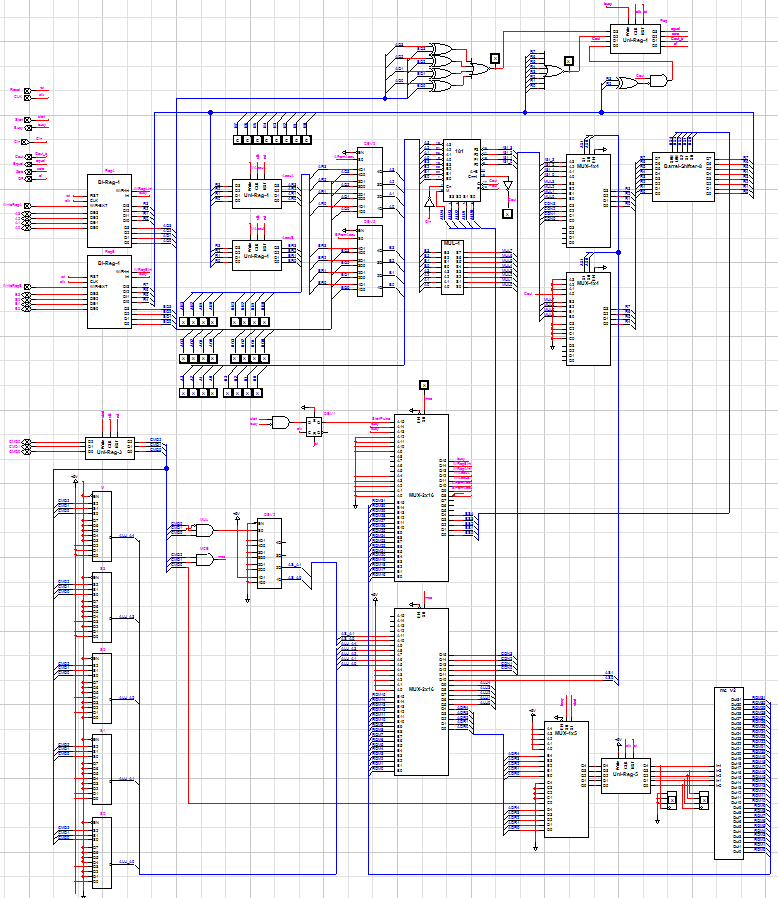
\includegraphics[width=\textwidth]{inneresBlockschaltbild}
			\label{inneresBlockschaltbild}
			\caption{Inneres Blockschaltbild}
		\end{center}
	\end{figure}
	
\end{document}